\eject
\newgeometry{margin=10mm}
\pdfpagewidth=300mm \pdfpageheight=210mm

\section{Atomic clock extensive comparison}
\label{appendix:atomic_clock}

\begin{table}[H]
    \centering
    \begin{tabular}{ll|lllllllllll}
        \hline
        \textbf{Vendor} & \textbf{Product} & \textbf{Type} & \textbf{ADEV} & \textbf{$\mathcal{L}$} & \textbf{Aging} & \textbf{Retrace} & \textbf{Tmin}          & \textbf{Tmax}          & \textbf{Tempco} & \textbf{Power} & \textbf{Weight} & \textbf{Size}           \\
        ~               & ~                & ~             & (1 s)         & (10 Hz)                & (month)        & ~                & (\textsuperscript{o}C) & (\textsuperscript{o}C) & ~               & (W)            & (kg)            & (cm\textsuperscript{3}) \\
        \hline
        Muquans         & MuC10ck          & cold Rb       & 3,00E-13      & -151                   & ~              & ~                & ~                      & ~                      & ~               & 200,00         & 135,000         & 682000                  \\
        T4Science       & iMaser-3000      & Maser         & 6,00E-14      & -136                   & 6,00E-15       & ~                & ~                      & ~                      & ~               & 100,00         & 100,000         & 436800                  \\
        Microsemi       & MHM 2020         & Maser         & 8,00E-14      & -138                   & 9,00E-15       & ~                & ~                      & ~                      & ~               & 75,00          & 246,000         & 374072                  \\
        Vremya          & VCH-1003M        & Maser         & 6,00E-14      & -135                   & 9,00E-15       & ~                & ~                      & ~                      & ~               & 100,00         & 100,000         & 305525                  \\
        T4Science       & pHMaser          & PHM           & 5,00E-13      & -130                   & 6,00E-14       & ~                & ~                      & ~                      & ~               & 90,00          & 33,000          & 49820                   \\
        Chengdu Spaceon & TA1000           & OPC           & 1,20E-11      & -125                   & ~              & ~                & ~                      & ~                      & ~               & 100,00         & 40,000          & 48266                   \\
        Spectradynamics & c-Rb             & cold Rb       & 5,00E-13      & -138                   & ~              & ~                & ~                      & ~                      & ~               & 75,00          & 30,500          & 39806                   \\
        Microsemi       & 5071A            & CBT           & 5,00E-12      & -130                   & ~              & ~                & 0                      & 55                     & ~               & 50,00          & 30,000          & 29700                   \\
        Oscilloquartz   & OSA 3235B Cs     & CBT           & 1,20E-11      & -120                   & ~              & ~                & ~                      & ~                      & ~               & 60,00          & 15,000          & 23021                   \\
        Microsemi       & cslll 4310B      & CBT           & 1,20E-11      & -130                   & ~              & ~                & 0                      & 50                     & ~               & 30,00          & 13,500          & 16544                   \\
        FEI             & FEI RAFS         & Space Rb      & 6,00E-13      & -138                   & 9,00E-13       & 5,00E-12         & -4                     & 25                     & ~               & 39,00          & 7,500           & 4902                    \\
        Spectratime     & iSpace RAFS      & Space Rb      & 3,00E-12      & -120                   & 8,30E-12       & ~                & -5                     & 10                     & ~               & 35,00          & 3,400           & 3224                    \\
        Excelitas       & RAFS             & space Rb      & 2,00E-12      & -105                   & 3,00E-12       & 5,00E-12         & -20                    & 45                     & ~               & 39,00          & 6,350           & 1645                    \\
        FEI             & FE-5669          & Rb            & 6,00E-12      & -140                   & 1,00E-11       & 2,00E-11         & -20                    & 60                     & 5,00E-11        & 20,00          & 1,690           & 669                     \\
        Microchip       & XPRO (low drift) & Rb            & 1,00E-11      & -90                    & 1,00E-11       & 3,00E-11         & -25                    & 70                     & 6,00E-10        & 13,00          & 0,500           & 455                     \\
        Spectratime     & miniRAFS         & Rb            & 1,00E-11      & -84                    & 3,00E-11       & ~                & -15                    & 55                     & ~               & 10,00          & 0,450           & 388                     \\
        IQD             & IQRB-2           & Rb            & 2,00E-12      & -138                   & 4,00E-11       & 2,00E-11         & ~                      & ~                      & ~               & 6,00           & 0,220           & 230                     \\
        Spectratime     & LP Rb            & Rb            & 1,00E-11      & -100                   & 3,00E-11       & 5,00E-11         & -25                    & 55                     & 2,00E-10        & 10,00          & 0,290           & 216                     \\
        SRS             & PRS10            & Rb            & 2,00E-11      & -130                   & 5,00E-11       & 5,00E-11         & -20                    & 65                     & 2,00E-10        & 14,40          & 0,600           & 155                     \\
        Accubeat        & AR133A           & Rb            & 5,00E-12      & -116                   & 1,00E-11       & 5,00E-11         & -20                    & 65                     & 1,00E-10        & 8,25           & 0,295           & 146                     \\
        IQD             & IQRB-1           & Rb            & 5,00E-11      & -95                    & 5,00E-11       & 2,00E-11         & 0                      & 50                     & 5,00E-10        & 6,00           & 0,105           & 66                      \\
        Chengdu Spaceon & XHTF1031 Rb      & CPT           & 5,00E-11      & -95                    & 5,00E-11       & ~                & -30                    & 65                     & 2,00E-10        & 6,00           & 0,200           & 65                      \\
        Spectratime     & mRO-50 (EAS)     & CSAC          & 4,00E-11      & -76                    & 1,50E-10       & 1,00E-10         & -10                    & 65                     & 4,00E-10        & 0,36           & 0,075           & 50                      \\
        Microsemi       & SA55 MAC         & CPT           & 3,00E-11      & -87                    & 5,00E-11       & 5,00E-11         & -10                    & 75                     & 5,00E-11        & 6,30           & 0,100           & 46                      \\
        Accubeat        & NAC              & CSAC          & 2,00E-10      & -86                    & 3,00E-10       & ~                & -20                    & 65                     & 2,00E-09        & 1,20           & 0,075           & 32                      \\
        Chengdu Spaceon & CPT              & CSAC          & 2,00E-10      & -90                    & 9,00E-10       & 5,00E-11         & -45                    & 70                     & 5,00E-10        & 1,60           & 0,045           & 24                      \\
        Teledyne        & TCSAC            & CSAC          & 3,00E-10      & -85                    & 3,00E-10       & 3,00E-10         & -10                    & 60                     & 1,00E-09        & 0,18           & 0,042           & 23                      \\
        Microsemi       & SA45.s           & CSAC          & 3,00E-10      & -70                    & 9,00E-10       & 5,00E-10         & -10                    & 70                     & 1,00E-09        & 0,12           & 0,035           & 17                      \\
        Microsemi       & SA65             & CSAC          & 3,00E-10      & -64                    & 9,00E-10       & 5,00E-10         & -40                    & 80                     & 3,00E-10        & 0,12           & 0,035           & 16                      \\
        \hline
    \end{tabular}
    \caption{Performance parameter for some of the most common atomic clock. Source \cite{Marlow-Scherer}.}
\end{table}

\eject
\restoregeometry
\pdfpagewidth=210mm
\pdfpageheight=297mm


\section{Chip-Scale Atomic Clocks comparison}
\label{appendix:csac}

\begin{table}[H]
    \centering
    \begin{tabular}{l|llll}
        \hline
        \textbf{Manufacturer/Model} & \textbf{Country} & \textbf{ADEV} & \textbf{Power} & \textbf{Size}           \\
        ~                           & ~                & (1 s)         & (W)            & (cm\textsuperscript{3}) \\
        \hline
        Jackson Labs CSAC GPSDO     & US               & 1E-10         & 1,4            & 85                      \\
        Seiko Epson A06860LAN       & JP               & 3E-11         & 3,0            & 75                      \\
        Precision Test Systems RFS2 & UK               & 3E-11         & 6,0            & 65                      \\
        Quartziock El O-MRX         & UK               & 5E-11         & 6,0            & 65                      \\
        Microsemi MAC SA.3Xm        & US               & 3E-11         & 5,0            & 50                      \\
        Orolia Spectratime mRO-50   & CH/FR            & 4E-11         & 0,5            & 50                      \\
        Chengdu Spaceon XHTF1031    & China            & 5E-11         & 6,0            & 50                      \\
        Microsemi MAC SA.5X         & US               & 3E-11         & 6,3            & 47                      \\
        Accubeat NAC1               & Israel           & 2E-10         & 1,2            & 32                      \\
        IQD ICPT-1                  & UK               & 9E-11         & 1,7            & 25                      \\
        Chengdu Spaceon XHTF1040    & China            & 3E-10         & 1,6            & 24                      \\
        Teledyne TCSAC              & US               & 3E-10         & 0,2            & 23                      \\
        Microsemi SA45.s            & US               & 3E-10         & 0,1            & 17                      \\
        Chengdu Spaceon XHTF1045    & China            & 3E-10         & 0,3            & 17                      \\
        \hline
    \end{tabular}
    \caption{Key parameters of the most common CSACs. Source \cite{Travagnin}.}
\end{table}

\pagebreak
\section{Rubidium energy levels}
\label{appendix:Rubidium-energy-levels}

Here follows a more comprehensive description of the energy levels of $^{87}Rb$ isotopes, as shown in Figure \ref{fig:Rubidium-energy-levels}.
The hyperfine structure of the $5^2S_{1/2}$ and $5^2P_{1/2}$ states is due to the interaction between the nuclear magnetic moment and the electron magnetic moment.
The hyperfine structure of the $5^2P_{3/2}$ state is due to the interaction between the nuclear magnetic moment and the total angular momentum of the electron.
The $5^2S_{1/2}$ state has two hyperfine levels, $F=1$ and $F=2$, separated by $\Delta E_{hfs} = 6.834682610904(10) \text{GHz}$.

\begin{figure}[H]
    \centering
    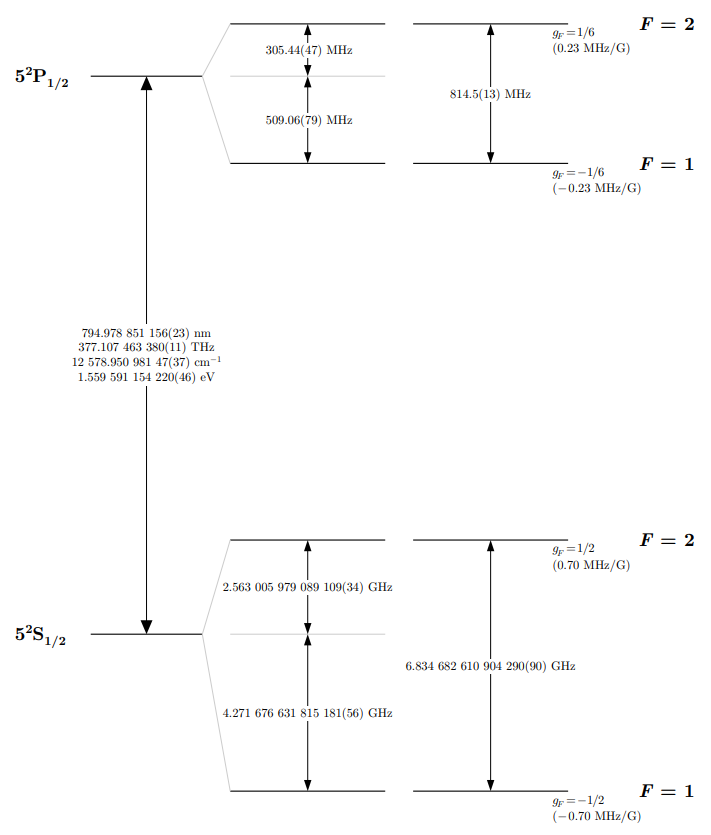
\includegraphics[width=0.9\textwidth, max width=\linewidth]{img/levels-Rubidium.png}
    \caption{Energy levels of $^{87}Rb$. Source \cite{ALKALINI}.}
    \label{fig:Rubidium-energy-levels}
\end{figure}

\pagebreak
\section{Cesium energy levels}
\label{appendix:Cesium-energy-levels}

Here follows a more comprehensive description of the energy levels of $^{133}Cs$ isotopes, as shown in Figure \ref{fig:Cesium-energy-levels}.
The hyperfine structure of the $6^2S_{1/2}$ and $6^2P_{1/2}$ states is due to the interaction between the nuclear magnetic moment and the electron magnetic moment.
The hyperfine structure of the $6^2P_{3/2}$ state is due to the interaction between the nuclear magnetic moment and the total angular momentum of the electron.
The $6^2S_{1/2}$ state has two hyperfine levels, $F=3$ and $F=4$, separated by $\Delta E_{hfs} = 9.192631770(10) \text{GHz}$.

\begin{figure}[H]
    \centering
    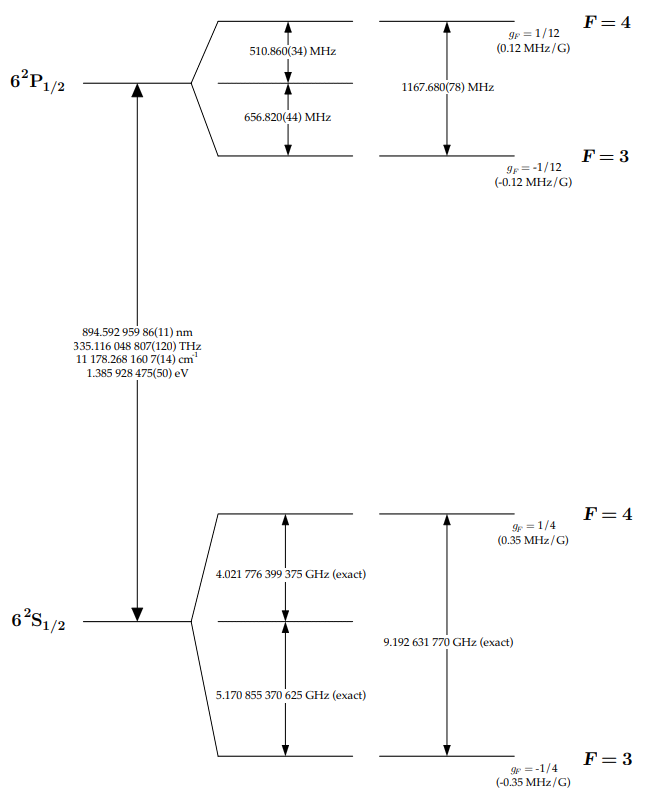
\includegraphics[width=0.9\textwidth, max width=\linewidth]{img/levels-Caesium.png}
    \caption{Energy levels of $^{87}Rb$. Source \cite{ALKALINI}.}
    \label{fig:Cesium-energy-levels}
\end{figure}


